%%%%%%%%%%%%%%%%%%%%%%%%%%%%%%%%%%%%%%%%
% Classe do documento
%%%%%%%%%%%%%%%%%%%%%%%%%%%%%%%%%%%%%%%%

% Nós usamos a classe "unb-cic".  Deixe apenas uma das linhas
% abaixo não-comentada, dependendo se você for do bacharelado ou
% da licenciatura.

\documentclass[bacharelado]{unb-cic}
%\documentclass[licenciatura]{unb-cic}



%%%%%%%%%%%%%%%%%%%%%%%%%%%%%%%%%%%%%%%%
% Pacotes importados
%%%%%%%%%%%%%%%%%%%%%%%%%%%%%%%%%%%%%%%%

\usepackage[brazil,american]{babel}
\usepackage[T1]{fontenc}
\usepackage{indentfirst}
\usepackage{natbib}
\usepackage{xcolor,graphicx,url}
\usepackage[utf8]{inputenc}
\usepackage{bm}
\usepackage{listings}
\usepackage{csquotes}
\usepackage{placeins}
\usepackage{amsmath}

%%%%%%%%%%%%%%%%%%%%%%%%%%%%%%%%%%%%%%%%
% Cores dos links
%%%%%%%%%%%%%%%%%%%%%%%%%%%%%%%%%%%%%%%%

% Veja o arquivos cores.tex se quiser ver que outras cores estão
% pré-definidas.  Utilizando o comando \hypersetup abaixo nós
% evitamos aquelas caixas vermelhas feias em volta dos links.

%%%%%%%%%%%%%%%%%%%%%%%%%%%%%%%%%%%%%%%%
% Cores do estilo Tango
%%%%%%%%%%%%%%%%%%%%%%%%%%%%%%%%%%%%%%%%

\definecolor{LightButter}{rgb}{0.98,0.91,0.31}
\definecolor{LightOrange}{rgb}{0.98,0.68,0.24}
\definecolor{LightChocolate}{rgb}{0.91,0.72,0.43}
\definecolor{LightChameleon}{rgb}{0.54,0.88,0.20}
\definecolor{LightSkyBlue}{rgb}{0.45,0.62,0.81}
\definecolor{LightPlum}{rgb}{0.68,0.50,0.66}
\definecolor{LightScarletRed}{rgb}{0.93,0.16,0.16}
\definecolor{Butter}{rgb}{0.93,0.86,0.25}
\definecolor{Orange}{rgb}{0.96,0.47,0.00}
\definecolor{Chocolate}{rgb}{0.75,0.49,0.07}
\definecolor{Chameleon}{rgb}{0.45,0.82,0.09}
\definecolor{SkyBlue}{rgb}{0.20,0.39,0.64}
\definecolor{Plum}{rgb}{0.46,0.31,0.48}
\definecolor{ScarletRed}{rgb}{0.80,0.00,0.00}
\definecolor{DarkButter}{rgb}{0.77,0.62,0.00}
\definecolor{DarkOrange}{rgb}{0.80,0.36,0.00}
\definecolor{DarkChocolate}{rgb}{0.56,0.35,0.01}
\definecolor{DarkChameleon}{rgb}{0.30,0.60,0.02}
\definecolor{DarkSkyBlue}{rgb}{0.12,0.29,0.53}
\definecolor{DarkPlum}{rgb}{0.36,0.21,0.40}
\definecolor{DarkScarletRed}{rgb}{0.64,0.00,0.00}
\definecolor{Aluminium1}{rgb}{0.93,0.93,0.92}
\definecolor{Aluminium2}{rgb}{0.82,0.84,0.81}
\definecolor{Aluminium3}{rgb}{0.73,0.74,0.71}
\definecolor{Aluminium4}{rgb}{0.53,0.54,0.52}
\definecolor{Aluminium5}{rgb}{0.33,0.34,0.32}
\definecolor{Aluminium6}{rgb}{0.18,0.20,0.21}

\hypersetup{
  colorlinks=true,
  linkcolor=DarkScarletRed,
  citecolor=DarkScarletRed,
  filecolor=DarkScarletRed,
  urlcolor= DarkScarletRed
}



%%%%%%%%%%%%%%%%%%%%%%%%%%%%%%%%%%%%%%%%
% Informações sobre a monografia
%%%%%%%%%%%%%%%%%%%%%%%%%%%%%%%%%%%%%%%%

\title{Armazenamento de Dados Abertos com NoSQL}

\orientador{\prof[a] \dr[a] Maristela Terto de Holanda}{CIC/UnB}
%\coorientador[a]{\prof[a] \dr[a] Coorientadora}{MAT/UnB}
\coordenador{\prof \dr Rodrigo Bonifácio de Almeida}{CIC/UnB}
\diamesano{15}{dezembro}{2016}

\membrobanca{\prof \dr Professor I}{CIC/UnB}
\membrobanca{\prof \dr Professor II}{CIC/UnB}

\autor{Jorge Luiz}{Andrade}
\CDU{004.4}

\palavraschave{bancos de dados, nosql, dados abertos }
\keywords{databases, nosql, open data}



%%%%%%%%%%%%%%%%%%%%%%%%%%%%%%%%%%%%%%%%
% Texto
%%%%%%%%%%%%%%%%%%%%%%%%%%%%%%%%%%%%%%%%

\begin{document}
  \maketitle
  \pretextual

  \begin{dedicatoria}
  Dedico a....
  \end{dedicatoria}

  \begin{agradecimentos}
  Agradeço a....
  \end{agradecimentos}

  \begin{resumo}
  A ciência...
  \end{resumo}

  \selectlanguage{american}
  \begin{abstract}
  The science...
  \end{abstract}
  %\selectlanguage{brazil}

  \tableofcontents
  \listoffigures
  \listoftables

  \textual
  \chapter{Introdução}

Dados abertos tem ganhado importância cada vez maior em nossa sociedade. O volume desses dados, que podem ser definidos como dados livres para acesso, utilização e modificação~\cite{opendefinition}, tem crescido cada vez mais, e vem sendo necessário encontrar novas formas para realizar o seu armazenamento e analise, comumente realizados por meio de bancos de dados.

Bancos de dados podem ser definidos como um conjunto de dados que se relazionam entre si e armazenados de forma que possam ser acessados posteriormente, quando necessario~\cite{leavitt2010nosql}.
Os bancos de dados relacionais predominaram por pelo menos nas últimas três décadas, mas seu desempenho em certas aplicações atuais, principalmente naquelas que trabalham com grande volumes de dados, denominado \emph{Big Data}, vem sendo questionado. 

Esse questionamento levou à criação do movimento NoSQL, um novo paradigma de armazenamento de dados que ignora certas restrições dos bancos relacionais tradicionais e tentam melhorar seu armazenamento e desempenho por meio de um sistema distribuído em \emph{clusters}.

A utilização de bancos NoSQL para o tratamento de grande volumes de dados provenientes de dados abertos é uma possibilidade a ser analisada, a fim de permitir um acesso mais fácil e rápido por parte da população. 









  \chapter{Dados Abertos}

O rápido crescimento no volume de dados gerados pela sociedade nos últimos anos tem levado à uma necessidade cada vez maior de ferramentas e pessoas que consigam trabalhar com esses dados. Um estudo da \emph{IDC Digital Universe}, realizado em 2011, estimou que naquele ano o volume de dados criados, replicados e consumidos foi de 1,8 trilhão de \emph{gigabytes}~\cite{gantz2012digital}. Esses dados, entretanto, não estão disponíveis de forma aberta ao público. Também não estão estruturados de forma que possam ser lidos e analisados por máquinas daqueles que possam acessá-los e manipulá-los~\cite{seijiconectados}. 

Nesse contexto, diversas empresas, governos e institutos vem trabalhando para uma maior abertura desses dados, objetivando os chamados dados abertos. O termo \enquote{Dados abertos} no conceito que conhecemos hoje surgiu em 1995 em um documento de uma agência científica americana no contexto da abertura de dados geofísicos e ambientais. Esse conceito vem sendo ampliado e estimulado nos últimos anos por diversos movimentos~\cite{seijiconectados}. 

A \emph{Open Definition} define um dado como aberto \enquote{se qualquer pessoa está livre para acessa-lo, utiliza-lo, modifica-lo, e compartilha-lo — restrito, no maximo, a medidas que preservam a proveniência e abertura.}~\cite{opendefinition}. A abertura dos dados evita mecanismos de controle e restrições sobre os mesmos, o que permite seu uso de forma livre~\cite{seijiconectados}.

A Open Knowledge Foundation, organização mundial que promove a abertura de dados~\cite{openknowledge}, resume esses pontos em:

\begin{itemize}
\item \textbf{Disponibilidade e Acesso}: os dados devem estar disponíveis como um todo e sob custo não maior que um custo razoável de reprodução, preferencialmente possíveis de serem baixados pela internet. Os dados devem também estar disponíveis de uma forma conveniente e modificável.

\item \textbf{Reutilização e Redistribuição}: os dados devem ser fornecidos sob termos que permitam a reutilização e a redistribuição, inclusive a combinação com outros conjuntos de dados.

\item \textbf{Participação Universal}: todos devem ser capazes de usar, reutilizar e redistribuir - não deve haver discriminação contra áreas de atuação ou contra pessoas ou grupos. Por exemplo, restrições de uso 'não-comercial' que impediriam o uso 'comercial', ou restrições de uso para certos fins (ex.: somente educativos) excluem determinados dados do conceito de 'aberto'.
\end{itemize}

\section{Classificação de Dados Abertos}
Tim Berners-Lee, o inventor da \emph{Web} e um defensor da abertura de dados, propõs, em 2010, princípios que definem um sistema de classicação de dados abertos por meio de estrelas. Quanto mais aberto é o dado, maior o número de estrelas que ele possui e mais fácil é para enriquece-lo~\cite{seijiconectados}.

As cinco estrelas de Tim Berners-Lee são:
\begin{itemize}
\item \textbf{1 estrela}: O dado está disponível na Internet, em qualquer formato, acompanhado de licença aberta.
\item \textbf{2 estrelas}: O dado está disponível na Internet de maneira estruturada, em um formato que permita sua leitura por máquinas (por exemplo, XML).
\item \textbf{3 estrelas}: O dado está disponível na Internet, de maneira estruturada, e em formato não proprietário (por exemplo, CSV).
\item \textbf{4 estrelas}: O dado está disponível na Internet, de maneira estruturada e em formato proprietário. Além disso, deve estar dentro dos padrões estabelecidos pela W3C (RDF): utilização de URI para nomear relações entre coisas e propriedades.
\item \textbf{5 estrelas}: Além das propriedades anteriores, ter no RDF conexões com com outros dados, por meio de \emph{links}, de forma a se obter um contexto de dados relevantes.
\end{itemize}

Dados publicados seguindo a classificação de estrelas de Berners-Lee conferem uma série de custos e benefícios, tanto para quem os publica quanto para quem os consome, sendo eles~\cite{seijiconectados}:
\begin{itemize} 
\item \textbf{1 Estrela}: 
	\item[] \textbf{Quem consome}
		\begin{itemize}
			\itemsep0em
			\item Ver os dados
			\item Imprimi-los
			\item Guardá-los
			\item Modificar os dados como queira
			\item Acessar os dados de qualquer sistema
			\item Compartilhar os dados com qualquer pessoa			
		\end{itemize}
		
	\item[] \textbf{Quem produz}
		\begin{itemize}
			\itemsep0em
			\item É simples de publicar
			\item Não é necessário explicar repetidamente para outros que eles podem usar seus dados
		\end{itemize}
		
\item \textbf{2 Estrelas}:

	\item[] \textbf{Quem consome}
		\begin{itemize}
			\itemsep0em
			\item É possível processa-los diretamente com\emph{softwares} proprietários 
			\item É possível exportar os dados para outro formato estruturado
		\end{itemize}
		
	\item[] \textbf{Quem produz}
		\begin{itemize}
			\itemsep0em
			\item Ainda é simples de publicar
		\end{itemize}

\item \textbf{3 Estrelas}:
	\item[] \textbf{Quem consome}
		\begin{itemize}
			\itemsep0em
			\item Você pode manipular os dados da forma que quiser, sem a necessidade de nenhum \emph{software} proprietário	
		\end{itemize}
		
	\item[] \textbf{Quem produz}
		\begin{itemize}
			\itemsep0em
			\item Ainda é relativamente simples de publicar
			\item Podem ser necessários \emph{plug-ins} ou conversores para exportar os dados do \emph{software} proprietário
		\end{itemize}
\item \textbf{4 Estrelas}:
	\item[] \textbf{Quem consome}
		\begin{itemize}
			\itemsep0em
			\item Fazer marcações nos dados
			\item Você pode reusar partes dos dados
			\item Você pode reusar ferramentas e bibliotecas existentes
			\item Você pode combinar os dados com outros dados
			\item O entendimento do formato RDF pode ser mais difício do que formatos tabulares (CSV) ou em árvore (XML).
			
		\end{itemize}
		
	\item[] \textbf{Quem produz}
		\begin{itemize}
			\itemsep0em
			\item Você tem um controle granular sobre seus dados, podendo realizar otimizações de acesso
			\item Outros publicadores de dados podem fazer ligações com seus dados
			\item Pode ser necessário investimento de tempo para dividir ou agrupar seus dados
			
		\end{itemize}
\item \textbf{5 Estrelas}:
	\item[] \textbf{Quem consome}
		\begin{itemize}
			\itemsep0em
			\item Você pode encontrar dados relacionados enquanto consome os dados
			\item Você pode aprender sobre o esquema de dados	
		\end{itemize}
		
	\item[] \textbf{Quem produz}
		\begin{itemize}
			\itemsep0em
			\item Os dados podem ser encontrados com maior facilidade
			\item Os dados possuem maior valor agregado
			\item A organização ganha os mesmos benefícios da vinculação de dados que os consumidores
		\end{itemize}
\end{itemize}

\section{Dados abertos governamentais}
Dados governamentais, em específico, também podem ser fundamentados por três leis e oito princípios.

Em 2009 o especialista em políticas públicas e dados abertos, David Eaves, propôs as seguintes três leis dos dados abertos governamentais, que também podem ser aplicadas a dados abertos em geral~\cite{eaveslaws}:

\begin{enumerate}
\item Se o dado não pode ser encontrado e indexado na Web, ele não existe;

\item Se o dado não está disponível em um formato aberto e compreensível por máquinas, ele não pode ser reaproveitado;

\item Se algum dispositivo legal não permite que ele seja replicado, ele é inútil.

\end{enumerate}

Em 2007, um grupo de trinta especialistas em governo aberto, reunidos em Sebastopol, na California, definiu os oito princípios de dados governamentais abertos, sendo eles~\cite{opengovdata}:

\begin{itemize}
\item \textbf{Completos}: todos os dados públicos deve estar disponíveis. Dados públicos são dados que não estejam sujeitos a limitações válidas de privacidade, segurança ou privilégio.

\item \textbf{Primários}: os dados devem ser iguais aos coletados na fonte, no maior nível possível de granularidade, não estando em formas agregadas ou modificadas.

\item \textbf{Atuais}: os dados devem ser disponibilizados tão rápido quanto necessário para garantir o seu valor.

\item \textbf{Acessíveis}: os dados devem ser disponibilizados para os mais amplos públicos e propósitos possíveis.

\item \textbf{Processáveis por máquinas}: os dados devem estar estruturados de forma razoável, de forma que permita um processamento automatizado.

\item \textbf{Não discriminatórios}: os dados devem estar disponíveis para todos, sem necessidade de registro ou identificação do usuário.

\item \textbf{Não proprietários}: os dados devem estar disponíveis em um formato que não seja controlado exclusivamente por uma entidade.

\item \textbf{Livres de licença}: os dados não devem estar sujeitos a qualquer restrições de direitos autorais, marcas, patentes ou segredos industriais. Restrições razoáveis de privacidade, segurança e privilégio podem ser permitidas.

\end{itemize}

\section{Contexto brasileiro de dados abertos}
A participação brasileira na área de dados abertos tem um marco em 2011 com a criação da \emph{Open Government Partnership}, uma aliança, contando inicialmente com a participação de 65 países, criada para fornecer uma plataforma internacional para reformadores nacionais comprometidos em fazer seus governos mais abertos, responsáveis e sensíveis aos cidadãos. Também foi criado o portal dados.gov.br, que disponibiliza dados governamentais de forma aberta~\cite{seijiconectados}.

O poder público brasileiro vem nos últimos anos realizando outras ações que promovem a abertura de dados governamentais. Essas ações visam benefícios como melhoria da gestão pública, transparência, controle a participação social, geração de emprego e renda e estímulo à inovação tecnológica~\cite{tcu}. Para atingir esse fim, no ano de 2012 foi definido, em instrução normativa, a implantação da INDA, Infraestrutura Nacional de Dados Abertos, \enquote{um conjunto de padrões, tecnologias, procedimentos e mecanismos de controle necessarios para atender às condições de disseminação e compartilhamento de dados e informações públicas no modelo de Dados Abertos}~\cite{inda}.  

O governo tem importância fundamental na questão de dados abertos, devido â grande quantidade de dados que coleta e por serem públicos, conforme a lei, podendo ser tornados abertos e disponíveis para a sociedade~\cite{openknowledge}.

Esses dados governamentais tem relevância tanto no âmbito da transparência, podendo haver rastreamento dos impostos e gastos governamentais; da vida pessoal, como na localização de serviços públicos por parte da população; economicamente, com a reutilização de dados abertos já disponíveis; e também dentro do próprio governo, que pode aumentar sua eficiência ao permitir que a população consulte diretamente dados que antes precisavam de interferência direta e individual por parte de funcionários públicos~\cite{openknowledge}.

Apesar desses esforços e da existência de programas avançados de transparência pública, ainda são raros os órgãos que disponibilizam dados de forma aberta. Em geral esses dados estão disponíveis para visualização, mas barreiras técnicas e políticas impedem sua reutilização~\cite{w3cmanual}.









  \chapter{Diferenças entre Bancos de Dados Relacionais e NoSQL}

O armazenamento a a manipulação de dados tem sido um importante foco da computação desde o seu nascimento, tendo os bancos de dados suas raízes ja na década de 60, principalmente em aplicações médicas e científicas~\cite{neufeld1986database}, e em 1970, Edgar Codd propos uma nova forma de armazenamento de dados, que ficou conhecida como modelo de dados relacionais (\emph{relational model of data})~\cite{codd1970relational}. 

\section{Bancos de Dados Relacionais}
    Podemos definir um banco de dados relacional como um conjunto de dados que se relacionam entre si e que são armazenados de forma persistente, podendo ser recuperados quando necessario. Os dados são armazenados em tabelas, que são organizadas por colunas, que definem uma categoria de um dado, e por linhas, que representam a instância de um dado~\cite{leavitt2010nosql}. A popularização desse modelo em virtude de suas características de persistência, concorrência e integração entre múltiplas aplicações, o transformou no modelo padrão de armazenamento computacional, principalmente em ambientes empresarias~\cite{pramod}. Outra questão de importância em bancos de dados computacionais é a não necessidade que o usuario tem de conhecer como esses dados são armazenados, o que foi possível com o uso dos chamados Sistemas Gerenciadores de Bancos de Dados (SGBDs)~\cite{jan}.
    
    Outras opções surgiram ao longo dos anos, como os bancos orientados a objetos ou bancos XML. Nenhum deles, entretanto, conseguiu competir com o modelo ja tradicional de dados relacionais.~\cite{pramod} Nos últimos anos, entretanto, o modelo conhecido como NoSQL vem surgindo como essa alternativa.
    
    Bancos de Dados relacionais tem como um de seus requisitos a existência de chaves primarias, colunas que que identificam unicamente cada linha, ou registro, de uma tabela. Um banco de dados relacional necessita de três informações para recuperar um dado específico: o nome da tabela, o nome da coluna e a chave primaria do registro que esta sendo buscado \cite{jan}.

\subsection{Propriedades ACID}
	Interações com bancos de dados relacionais tradicionais são feitas por meio de transações, que podem ser definidas como operações de leitura e escrita que devem ocorrer de forma independente umas das outras~\cite{dmsbook}. Para garantir que isso ocorra, um SGBD deve prover as seguintes propriedades, conhecidas como propriedades ACID~\cite{haerder}:
	\begin{itemize}
	\item \textbf{Atomicidade}, onde uma determinada transação deve ser feita em sua totalidade, ou seja, todas as operações de que dela fazem parte devem ser bem sucedidas.
	\item \textbf{Consistência} diz que após cada transação, o estado do banco permanece consistente ao seu modelo.
	\item \textbf{Isolamento} garante que cada transação é executada independentemente de outras que estejam ocorrendo em concorrência.
	\item \textbf{Durabilidade} que define que o resultado de uma transação bem sucedida é persistido no banco, mesmo na eventualidade de falhas no sistema.
	\end{itemize}

	Essas propriedades, ao mesmo tempo que garantem a validade do esquema e dos dados em um banco, sacrificam desempenho e disponibilidade, características importantes em varias aplicações atuais~\cite{foxcluster}.

\subsection{Normalização}
	Uma pratica comum e recomendada no projeto de bancos de dados relacionais é a normalização. O processo de normalização segue regras conhecidas como formas normais, onde cada forma normal representa um incremento desse conjunto de regras \cite{jan}. 
	Existem pelo menos seis formas normais, mas na maioria dos casos um banco é considerado bem projetado quando cumpre as exigências da terceira forma normal (3FN).

\subsection*{Primeira Forma Normal}
	Uma tabela esta na primeira forma normal (\textbf{1FN}) se cada tabela esta organizada por colunas e linhas, com cada linha possuindo uma chave primaria única que a identifica. 
	Além disso cada campo deve possuir apenas valores atômicos. Ou seja, cada coluna deve guardar apenas uma informação, não podendo existir listas ou conjuntos de valores dentro de uma mesma coluna de uma linha.

\subsection*{Segunda Forma Normal}
	Uma tabela esta na segunda forma normal (\textbf{2FN}) quando, além de obedecer à primeira forma normal, possui todos atributos não-chave funcionalmente dependentes da chave primaria. Dependência funcional é definida como uma relação entre dois atributos tal que para cada valor único do atributo A, existe apenas um valor do atributo B associado a ele~\cite{jan}. Em outras palavras, uma coluna não pode depender apenas de parte da chave primaria, ou seja, se uma tabela não possui chave primaria composta e esta na primeira forma normal, ela também esta na segunda forma normal.
	
\subsection*{Terceira Forma Normal}
	Uma tabela esta na terceira forma normal (\textbf{3FN}) quando, além de obedecer à segunda forma normal, não apresenta dependências transitivas, ou seja, cada atributo não-chave não pode ser determinado, ou dependente, de outro atributo não-chave. 

\section{Bancos NoSQL}
    O rapido crescimento no volume de dados nos últimos anos, principalmente após a bolha da Internet na década de 90~\cite{pramod}, tras uma necessidade de certa mudança em relação ao modelo tradicional. Modelos relacionais possuem diversas vantagem ja citadas, porém restrições como propriedades ACID e normalização, levam ao surgimento de problemas quando precisamos aplica-los nesse domínio recente de expansão dos dados, por apresentarem problemas de escalabilidade, complexidade dos dados e rigidez em seus esquemas~\cite{leavitt2010nosql}. 
    
    Isso levou ao surgimento de um movimento em direção ao novo paradigma denominado NoSQL. O termo foi utilizado pela primeira vez em 1998 para denominar um banco de dados que omitia o uso de SQL, o \emph{Strozzi NOSQL}. A definição atual, porém, tem suas bases em uma reunião, conhecida como \emph{NoSQL Meetup} realizada em 2009 em São Franscisco, Estados Unidos. Organizada por Johan Oskarsdon, criador do Last.fm, nela foram discutidas formas mais eficientes e baratas de organização dos dados, como as ja sugeridas em publicações anteriores, como o Google Bigtable em 2006~\cite{bigtable}, e Amazon's Dynamo em 2007~\cite{dynamo, chrisnosql}.
\subsection{Definição e Características}
Apesar do termo não tem uma definição precisa e universalmente aceita, sendo geralmente descrito como \emph{Not Only SQL}, bancos NoSQL em geral são caracterizados, mas não definidos, como sendo não relacionais, sem esquema bem definido, distribuidos e tolerantes a falhas~\cite{pramod}. Buscam um processamento de dados rápido e de forma eficiente, evitando a rigidez dos bancos tradicionais. 
	Entre as razões e vantagens dos bancos NoSQL podemos citar~\cite{chrisnosql}:
    \begin{itemize}
    \item \textbf{Evitar complexidade desnecessária}: Bancos relacionais costumam aderir às já citadas propriedades ACID, além de serem restritos em seu esquema de dados. Bancos NoSQL costumam ignorar ou relaxar essas restrições a fim de obter um melhor desempenho.
    \item \textbf{Alto rendimento}: Bancos NoSQL surgiram da necessidade e armazenamento e processamento de um cada vez maior volume de dados, e por isso são construídos objetivando um desempenho melhor, em aplicações específicas, do que de bancos tradicionais.
    \item \textbf{Alta escalabilidade}: Bancos relacionais podem ser escalados verticamente com a utilização de equipamentos poderosos e caros, e uma operação distribuida costuma ser mais complexa devido à forma de armazenamento de seus dados~\cite{leavitt2010nosql}. Bancos NoSQL foram pensados para execução em um sistema de \emph{clusters}, o que facilita a sua escalabilidade horizontal e reduz a necessidade de um hardware mais caro e específico, podendo ser utilizado em \emph{hardwares} mais simples. 
    \item \textbf{Alta disponibilidade}: Devido à possibilidade de escalabilidade horizontal, bancos NoSQL podem distribuir sua operação em diversos nós de um \emph{cluster}, o que possibilita acesso simultâneo por um grande número de usuários, mesmo que não seja possível acessar algum desses nós. 
    \item \textbf{\emph{Open source}}: SGBDs tradicionais costumam possuir licenças pagas, gerando um custo financeiro alto, principalmente quando executados em múltiplas maquinas~\cite{pramod}. NoSQLs costumam seguir licenças \emph{open source}, podendo reduzir significativamente os gastos da aplicação. 
\end{itemize}

\subsection{Teorema CAP}
\label{sec:cap}
	Em 2000 Eric Brewer, pesquisador na \emph{University of California}, propõs o teorema CAP, que define limitações em sistemas distribuidos. O teorema define que podemos garantir somente duas das seguintes três propriedades em um determinado sistema: Consistência (\emph{Consistency}) , Disponibilidade (\emph{Availability}) e Tolerância a partições (\emph{Partition-resilience})~\cite{brewer}. Essas propriedades podem ser definidas como:
    \begin{itemize}
	\item \textbf{Consistência} define que todos os nós possuem os mesmos dados em qualquer dado instante, e um pedido de leitura em qualquer desses nodos garante o dado mais atual possível do sistema.
    \item \textbf{Disponibilidade} garante é sempre possível ler e gravar dados em um nodo dado que ele esta acessível. 
    \item \textbf{Tolerância a partições} garante que o sistema ira continuar funcionando mesmo na hipótese de eventuais falhas de comunicação entre os nodos.
	\end{itemize}
	
    Essas propriedades podem ser agrupadas da seguinte forma e obtendo os seguintes resultados:
    \begin{itemize}
    \item \textbf{CA} são sistemas distribuídos cujos nós estejam em uma mesma partição de rede.
    \item \textbf{CP} são sistemas que, em caso de falha em pelo menos um dos nós, ficam indisponíveis até sua total recuperação. Bancos de Dados que seguem as propriedades ACID costumam seguir esse padrão.
    \item \textbf{AP} são sistemas que devem permanecer em funcionamento mesmo durante uma eventual falha em um ou mais de seus nós, mesmo que isso resulte em dados não atualizados durante consultas. Sistemas NoSQL costumam seguir esse padrão.  
	\end{itemize}
    
    Sistemas distribuídos, entretanto, por estarem sempre sujeitos a falhas de rede~\cite{deutsch}, não podem ignorar a Tolerância a Falhas, tendo de fazer uma escolha entre Consistência e Disponibilidade~\cite{brewer12years}.
    
    A figura~\ref{fig:capnosql} ilustra as diferentes combinações das propriedades CAP e exemplos de bancos de dados que as utilizam.
    

\begin{figure}[!htb]
\centering
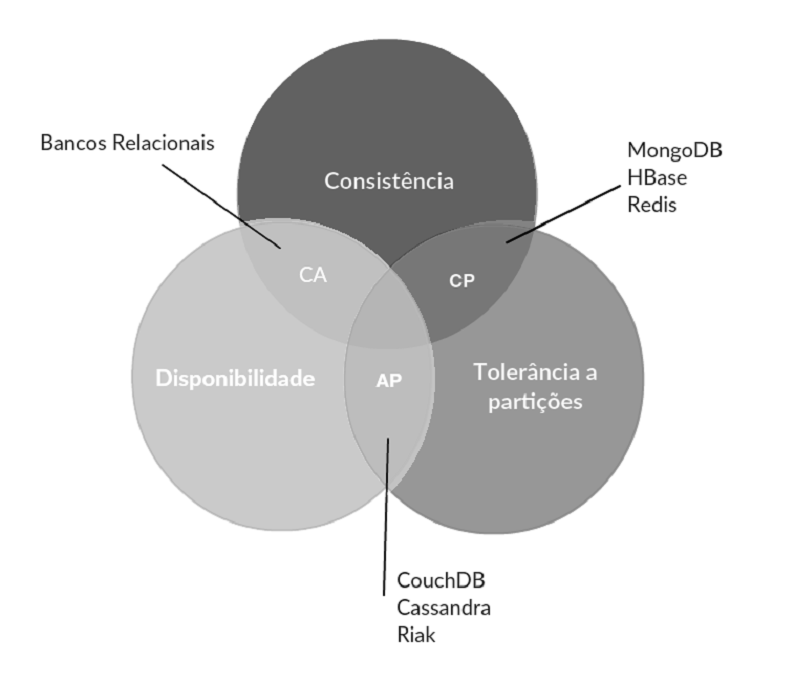
\includegraphics[width=0.7\textwidth]{figuras/cappb.png}
\caption{Propriedades CAP e exemplos. Adaptado de ~\cite{blograshid}}
\label{fig:capnosql}
\end{figure}

\subsection{BASE}
    Em um ambiente distribuido, escabalibilidade, resiliência e velocidade são mais importantes do que consistência imediata e segurança quanto à veracidade dos  dados, não sendo necessaria a aderência total às propriedades ACID ja citadas~\cite{neo4j_acidbase}. Além disso, de acordo com o \textbf{Teorema CAP}, um banco que aceite particionamento não pode possuir alta disponibilidade e consistência simultâneamente. Essa necessidade, tanto de performance quanto de disponibilidade, levou à criação do acrônimo \textbf{BASE}, \emph{\textbf{B}asically \textbf{A}vailable} (Basicamente Disponível), \emph{\textbf{S}oft State} (Estado Leve) e \emph{\textbf{E}ventual Consistency} (Consistência Eventual)~\cite{foxcluster}. 
    
    Enquanto um banco \textbf{ACID} é pessimista, requerendo que cada operação mantenha a consistência do banco como um todo, \textbf{BASE} segue uma visão otimista, entendendo que dados serão eventualmente consistentes.
    
    Sistemas distribuídos costumam manter cópias de dados em varias maquinas em um \emph{cluster} para aumentar a sua disponibilidade, e quando um desses dados é atualizado em uma dessas maquinas é natural que haja um intervalo de tempo até que todas essas cópias sejam atualizadas.

\subsection{Modelos NoSQL}
Bancos de dados NoSQL possuem padrões de modelos de dados, que compartilham certas características em comum e servem a determinadas aplicações específicas, podendo alguns bancos serem classificados em mais de uma categoria. A tabela ~\ref{tab:modelosnosql} lista os quatro modelos atuais e alguns bancos de dados que se enquadram em cada um deles.

~\begin{table}[]
\centering
\caption{Modelos de Bancos NoSQL}
\label{tab:modelosnosql}
\begin{tabular}{ll}
\textbf{Modelo de Dados}     & \textbf{Exemplo de bancos de dados}      \\ \hline
Chave-Valor         & Project Voldemort               \\
                    & Riak                            \\
                    & Redis                           \\
                    & BerkeleyDB                      \\ \hline
Documentos          & CouchDB                         \\
                    & MongoDB                         \\
                    & OrientDB                        \\ \hline
Famílias de colunas & Cassandra                       \\
					& Hypertable                      \\
                    & HBase                           \\ \hline
Grafos              & Neo4j \\
                    & OrientDB                        \\
                    & Infinite Graph                 
\end{tabular}
\end{table}

\subsection*{Chave-Valor}
Bancos com armazenamento em chave-valor existem a muito tempo, como \emph{Berkeley DB}, mas ganharam importância no meio NoSQL a partir do Amazon DynamoDB e do Google BigTable~\cite{chrisnosql}.

Consiste basicamente em uma tabela \emph{hash}, sendo o acesso aos dados realizado por meio de uma chave primaria, assim como ocorre em \emph{maps} e dicionarios.  Esses bancos são completamente livres de esquema e suas operações se resumem a consultar o valor a partir de uma chave, inserir um valor para uma chave ou deletar uma chave e seu valor do banco~\cite{nosqleval}. O valor armazenado em geral pode representar qualquer tipo de objeto, como uma \emph{string} ou um \emph{BLOB}, não sendo necessária que exista qualquer relação entre diferentes registros, ficando a aplicação responsável pelo seu tratamento. 

Esses bancos favorecem escalabilidade sobre consistência, e por isso em geral não possuem ferramentas mais poderosas de consulta e analise de dados~\cite{chrisnosql}.

Atualmente temos como exemplos de bancos chave-valor: \emph{Riak}, \emph{Redis}, \emph{Berkeley DB} e \emph{Project Voldemort}.

\subsection*{Documentos}
Bancos orientados a documentos armazenam seus dados em forma de documentos, podendo esses terem formato \emph{XML}, \emph{JSON}, \emph{BSON}, etc~\cite{pramod}. Podem ser vistos como a sequência natural do armazenamento por chave-valor, ainda fazendo o armazenamento por meio de um par chave-valor, mas utilizando uma estrutura mais rica para armazenamento dos dados ao armazenar um documento na parte do valor~\cite{chrisnosql}. Cada um desses documentos pode ter certa semelhança uns com os outros, mas não necessitam possuir a mesma estrutura, o que permite uma grande flexibilidade no esquema do banco.

A seguir temos um exemplo de dois documentos. Apesar de parecidos, eles possuem certas diferenças, o que gera essa grande flexibilidade do modelo orientado a documentos.

\begin{lstlisting}
{
  "clienteid" : "f6a6fs86fa",
  "cliente" :
  {
    "primeironome" : "Pedro",
    "sobrenome" : "Silva", 
    "gosta" : ["Leitura", "Viagem"]
  }
  "endereco" : 
  {
    "estado" : "Sao Paulo",
    "cidade" : "Guarulhos"
  }
}

{
  "clienteid" : "ga9s8g8fe",
  "cliente" :
  {
    "primeironome" : "Maria",
    "sobrenome" : "Costa", 
    "gosta" : ["Esportes"]
  }
  "ultimaCompra" : "12/11/2015"
}
\end{lstlisting}

Esses documentos não são opacos à aplicação, seu conteúdo pode ser consultado diretamente, com consultas diretas em atributos de seus registros. Isso permite a manipulação de estruturas mais complexas, que ainda assim não possuem nenhuma restrição de esquema, sendo facil a inserção de novos documentos ou a modificação dos documentos ja armazenados. Devido à essa flexibilidade, são recomendados para integração de dados e migração de esquemas~\cite{nosqleval}. 

Como exemplos de bancos orientados a documentos podemos citar o \emph{CouchDB}, \emph{MongoDB} e \emph{OrientDB}.

\subsection*{Colunas}
Bancos de Dados colunares tem sua influência no \emph{Google BigTable}~\cite{bigtable}, e armazenam seus dados em famílias de colunas que são associadas a uma chave de linha. Cada uma dessas famílias de colunas pode possuir varias colunas, e são consideradas dados relacionados que podem ser acessados ao mesmo tempo~\cite{pramod}. 

O Cassandra possui ainda o conceito de super colunas, que pode ser visto como um agrupamento de colunas que pode ser armazenado dentro de uma família de colunas~\cite{pramod}.

Colunas e linhas podem ser adicionadas a qualquer momento, o que gera uma flexibilidade bem maior em relação aos esquemas em geral fixos dos bancos de dados relacionais.  Entretanto, famílias de colunas em geral devem ser predefinidas, situação menos flexível que a encontrada nos modelos de chave-valor ou de documentos~\cite{nosqleval}.  

Como exemplo de bancos orientados a colunas temos o \emph{HBase} e \emph{Hypertable}, que são implementações \emph{open source} do BigTable, e o \emph{Cassandra}.


\subsection*{Grafos}
Diferente dos bancos relacionais e dos ja citados modelos NoSQL vistos, um banco de dados em grafos é especializado em dados altamente conectados. São ideias para aplicações que realizam consultas baseadas em relações~\cite{nosqleval}.
Esse modelo realiza o armazenamento por meio de entidades e os relacionamentos entre essas entidades. Entidades podem ser vistas como nós e os relacionamentos como as areas de um grafo~\cite{pramod}. Esses nós podem possuir propriedades dos objetos que representam, assim como as áreas, que podem possuir atributos do relacionamento e além disso possuem significância em sua direção.

Consultas nesse tipo de modelo são realizadas percorrendo o grafo. Isso possui como vantagem a possibilidade de se modificar a forma que se camanha nesse grafo, sem ser necessarias mudanças em sua estrutura de nós e relações~\cite{pramod}.

Uma diferença importante dos bancos orientados a grafos em relação aos modelos anteriores é o seu suporte menor a sistemas distribuidos, não sendo geralmente possível a distribuição dos nós em diferentes servidores~\cite{pramod}.

Como exemplos desse modelo podemos citar o \emph{Neo4J}, o \emph{Infinite Graph} e o \emph{OrientDB}.
  \chapter{Cassandra}

Esse trabalho ira utilizar o Cassandra como banco de dados para validação de sua hipótese. Como visto no capítulo 3, o Apache Cassandra, distribuição que sera utilizada, é um banco de dados orientado a colunas altamente disponível e distribuído em servidores constituídos de hardware de \enquote{prateleira} para gerenciamento de grande volumes de dados~\cite{lakshmancassandra}. Este capítulo tem como objetivo definir esse banco de dados, suas características, funcionamento, vantagens e desvantagens.

\section{Definição}
O Cassandra se originou em 2007 como um projeto do \emph{Facebook} para resolver um problema na busca da caixa de mensagens. A compania necessitava de um sistema com alta performance, confiabilidade, eficiência e que suportasse o contínuo crescimento da ferramenta~\cite{lakshmancassandra, cassandraguide}. 

O projeto foi desenvolvido por Jeff Hammerbacher, Avinash Lakshman, Karthik Ranganathan e Prashant Malik, tendo seu modelo de dados sofrido grande inspiração nos trabalhos anteriores do \emph{Amazon Dynamo}~\cite{dynamo} e do \emph{Google Bigtable}~\cite{bigtable}, e lançado em 2008 como um projeto \emph{open source}. Foi mantido e atualizado apenas pelo Facebook até 2009, quando foi comprado pela Apache~\cite{cassandraguide}, sendo utilizado atualmente por companias como \emph{Netflix}, \emph{Spotify} e até em agências governamentais, como a NASA~\cite{cassandracompanies}. 

O Apache Cassandra pode ser definido como um banco de dados orientado a colunas \emph{open source}, distribuído, descentralizado, elasticamente escalavel, altamente disponível, tolerante a falhas e variavelmente consistente~\cite{cassandraguide}. A seguir iremos analisar cada uma dessas características.

\subsection{Características}

\subsection*{Distribuído e Descentralizado}
O Cassandra é capaz de ser executado em múltiplas de forma transparente ao usuário, que o enxerga como um sistema unificado. Apesar de ser possível sua execução em um único nó, só é possível obter algum benefício com uma execução distribuída. Além do ganho de performance, a distributividade do sistema garante maior segurança devido à redundância de dados.

Diferente de outros bancos distribuídos que elegem nós como mestres e escravos, o Cassandra opera de forma descentralizada, o que significa que todos os nós são idênticos em sua forma de execução, sendo utilizados protocolos \emph{peer-to-peer} (par-a-par) e \emph{gossip} para manutenção e sincronia entre os nós. Essa descentralização garante que não exista apenas um ponto de falha, o que aumenta sua disponibilidade, e simplifica a operação do e manutenção do \emph{cluster}.

\subsection*{Elasticamente Escalável}
Escalabilidade é a propriedade que um sistema tem de atender um crescente número de requisições sem prejuízo de performance. Essa escalabilidade pode ser tanto vertical quanto horizontal. Na escalabilidade vertical o hardware já utilizado no sistema é melhorado, enquanto na escalabilidade horizontal novos máquinas são adicionadas à arquitetura, havendo a divisão da carga do sistema.

O Cassandra possui escalabilidade horizontal elástica, o que significa que sua arquitetura pode escalar tanto para cima quanto para baixo. Na necessidade de uma melhora do desempenho da aplicação, novas máquinas podem ser adicionadas, e o Cassandra se encarrega de fazer a distribuição dos dados de forma transparente, sem necessidade de configurações adicionais ou reiniciamento do sistema. Da mesma forma, em caso de necessidade, máquinas podem ser retiradas do \emph{cluster} sem prejuízo ao todo, devido ao rebalanceamento automático.

\subsection*{Altamente disponível e Tolerante a falhas}
A disponibilidade de um sistema é medida de acordo com sua capacidade de responder a requisições. Computadores, e especialmente sistemas distribuídos em rede, estão sujeitos a falhas, que em geral só podem ser contornadas por meio de sistemas redundantes.

Devido a replicação e redundância de dados e a sua capacidade de substituição de nós indisponíveis, o Cassandra pode ser definido como um sistema altamente disponível e tolerante à falhas em suas máquinas.

\subsection*{Variavelmente Consistente}
A consistência de uma aplicação diz respeito à sua capacidade de retornar o valor mais atual em uma requisição.

Como visto no Teorema CAP~\ref{sec:cap}, não é possível a um sistema ser totalmente consistente, disponível e tolerante a falhas. 

O Cassandra é por vezes definido como \enquote{eventualmente consistente}, por trocar parte de sua consistência por alta disponibilidade. Essa definição, porém, não é totalmente correta, e um termo melhor para defini-lo é \enquote{variavelmente consistente} (\emph{tuneably consistent}), podendo essa sua consistência ser ajustada de acordo com o tipo de aplicação.

\section{Modelo de Dados}

Um banco de dados Cassandra consiste em um \emph{keyspace} contendo famílias de colunas, que por sua vez definem um conjunto de linhas que englobam várias colunas. Essa disposição de dados é bastante semelhante ao que foi proposto pelo Bigtable~\cite{lakshmancassandra, bigtable}. Seu modelo de dados pode ser visto como um mapa multidimensional indexado por uma chave, se assemelhando aos modelos de chave-valor e orientados à colunas. A seguir veremos em detalhes cada um desses conceitos.

A figura \ref{fig:cassandradm} ilustra de forma resumida o modelo de dados do Cassandra, contendo um \emph{keyspace} e seus componentes. 

\begin{figure}[!htb]
\centering
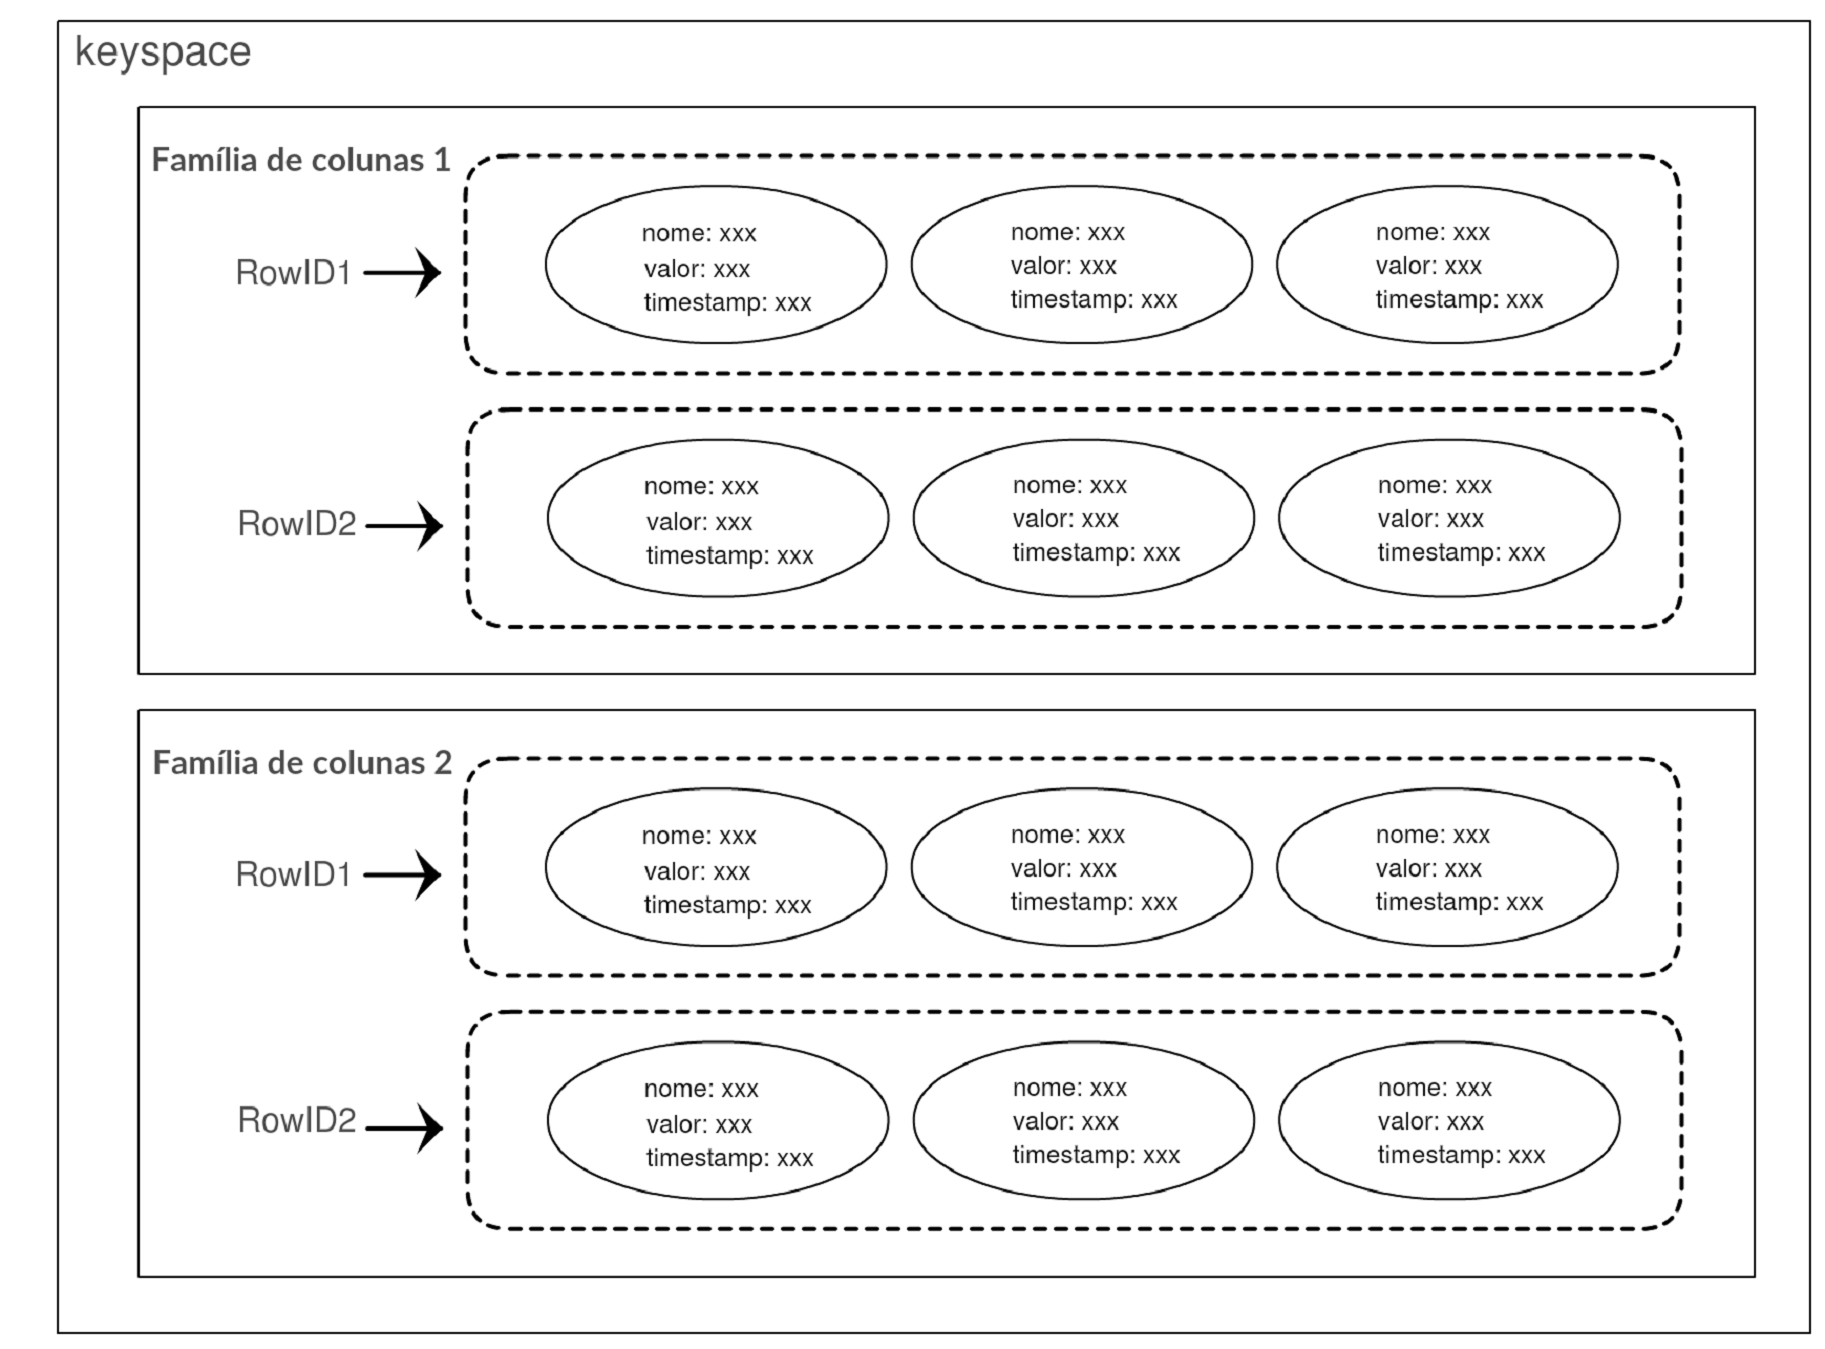
\includegraphics[width=1\textwidth]{figuras/cassandradatamodel.png}
\caption{Modelo de dados do Cassandra. Adaptado de ~\cite{ibmcassandra}}
\label{fig:cassandradm}
\end{figure}

\subsection*{\emph{Keyspace}}
Um \emph{keyspace} define o agrupamento de dados mais externo no Cassandra, podendo ser correspondido a um banco de um SGBD relacional. Um \emph{keyspace} define um nome e uma série de atributos que definem o seu comportamento. 
Atributos do \emph{keyspace} incluem~\cite{cassandraguide}:
\begin{itemize}
\item \textbf{Fator de replicação} diz respeito ao número de nós que armazenarão uma réplica de cada linha de dados. O fator de replicação tem forte influencia no balanço entre performance e consistência do banco de dados.
\item \textbf{Estratégia de replicação} se refere a como as réplicas (ou cópias) de um dado serão posicionados no anel do \emph{cluster}. Diversas estratégias de replicação estão disponíveis no Cassandra.
\item \textbf{Famílias de colunas} pode ser visto como o análogo às tabelas de um modelo relacional, da mesma forma que o \emph{keyspace} é o análogo do banco.  Uma família de colunas é um agrupamento para uma coleção de linhas, onde cada linha contém colunas ordenadas.
\end{itemize}



\subsection*{Colunas e famílias de colunas}
Uma família de colunas (ou tabela) no Cassandra é um mapa multidimensional indexado por uma chave. Essa chave é uma \emph{string} sem restrição de tamanho, mas que em geral varia de 16 a 36 \emph{bytes}. O valor desse mapeamento consiste em uma família de colunas, um agrupamento para uma coleção ordenadas de linhas, que por sua vez é uma coleção ordenada de colunas ~\cite{lakshmancassandra, cassandraguide}.

Uma família de colunas possui dois atributos: um nome e um comparador. O nome identifica a coluna para realização de consultas, enquanto o comparador indica como as colunas serão ordenadas ao serem retornadas em uma consultas, podendo ser \emph{long}, \emph{byte}, UTF8, etc~\cite{cassandraguide}.

O modelo de família de colunas se diferencia do modelo relacional por ser o que é chamado comumente de \emph{livre de esquema} (\emph{schema free}) . É possível realizar a inserção, remoção ou alteração de qualquer coluna ou família de colunas a qualquer momento, ficando as aplicações clientes do banco encarregadas de interpretar e manipular o novo modelo de dados. 

Ao se inserir um novo dado em uma família de colunas do Cassandra são especificados valores para uma ou mais colunas. O conjunto de valores é chamado de linha, e é identificado unicamente por uma chave primária ou chave de linha. Uma linha não precisa possuir dados para todas colunas presentes na família de colunas à que ela pertence, sendo o espaço alocado apenas para as colunas presentes nessa linha. Isso gera tanto uma economia de espaço quanto uma melhora de performance em relação a um banco relacional, que precisa preencher com valores nulos colunas não utilizadas.

Uma coluna é a unidade básica de armazenamento do Cassandra, e é constituida por um nome, um valor e um \emph{timestamp}. Se difere do conceito de colunas de bancos relacionais pois durante a criação do banco não é necessário a criação de colunas, e sim apenas famílias de colunas. A criação de colunas ocorre apenas durante a inserção de dados no banco e suas colunas correspondentes~\cite{cassandraguide}.

\section{Arquitetura}

O Cassandra foi projetado para lidar com grandes massas de dados distribuídas em vários nós sem ponto único de falha, pensado no fato de que tanto um sistema quanto componentes de hardware podem falhar.
Ao contrário de outras soluções de bancos de dados distribuidos, sejam elas relacionais ou modelos mais novos como o \emph{Google Bigtable}, em que os nós são definidos como mestres e escravos (\emph{master} e \emph{slave}), a arquitetura Cassandra combate o problema de falhas ao empregar uma distribuição par-a-par (\emph{peer-to-peer}) entre nós estruturalmente idênticos, com dados distribuidos entre todos os nós de um \emph{cluster}~\cite{cassandradocs, cassandraguide}.  

Essa decisão arquitetural de nós atuando de maneira par-a-par tem como objetivo melhorar a disponibilidade e facilidade de escalamento do sistema. Na ocasião de um nó ficar indisponível, existe um potencial impacto na vazão de dados do sistema, entretanto isso não causa uma interrupção no serviço. 
Ao mesmo tempo, ao se inserir um novo nó no sistema, é necessário que ele recebe informações sobre a topologia do anel em que está inserido e dados que ele será responsável. Após isso, entretanto, ele pode integrar o anel e receber requisições assim como os outros nós, sem necessidade de configurações complexas~\cite{cassandraguide}.

O Cassandra é um banco de dados particionado em linhas, com cada linha organizada em tabelas com uma chave primária obrigatória. Sua arquitetura permite que qualquer usuário autorizado se conecte a qualquer nó em qualquer \emph{data center} e acesse os dados por meio da linguagem \emph{CQL}, que possui sintaxe próxima a do \emph{SQL}, com abstração de uma tabela com linhas e colunas~\cite{cassandradocs}. 

Requisições de leitura e escrita podem ser enviadas a qualquer nó do \emph{cluster}, devido à característica de homogeneidade entre eles. Ao realizar uma conexão com um cliente, o nó atua como coordenador dessa operação, servindo de ponte entre a aplicação e os nós que possuem o dado requisitado. O coordenador também determina quais nós devem receber a requisição de acordo com a configuração do \emph{cluster}~\cite{cassandradocs}. 

\subsection{Protocolo Gossip}

Cada nó frequentemente troca informações de estado sobre ele mesmo e outros nós do cluster utilizando um  protocolo \emph{gossip}. \emph{Gossip} é um protocolo de comunicação par-a-par em que os nós realizam  troca de informações periódicas sobre o estados eles mesmos e sobre outros nós do \emph{cluster} de que eles tem conhecimento. Seu nome vem do conceito humano de \enquote{fofoca} (\emph{gossip}), uma forma de comunicação em que cada par pode escolher com quem ele deseja trocar informações~\cite{cassandradocs, cassandraguide}. 

Protocolos \emph{gossip} em geral assumem uma rede falha, e são em geral utilizados em sistemas em rede grandes e descentralizados, em geral em mecanismos de replicação em bancos de dados~\cite{cassandraguide}. 

O processo \emph{gossip} executa a cada segundo, e troca mensagens de estado com até três outros nós no \emph{cluster}. Uma mensagem \emph{gossip} tem uma versão associada a ela, de forma que durante sua troca, informações obsoletas são reescritas com o estado mais atual do nó em questão.

Para evitar problemas na comunicação \emph{gossip}, deve-se utilizar uma mesma lista de nós \emph{seed} para todos os nós do \emph{cluster}. Um nó \emph{seed} é aquele que mantem informações sobre todos os nós da rede. Por padrão, um nó lembra outros nós com quem ele tenha trocada informações entre reinícios do sistema, o nó \emph{seed} tem como única função inicializar o processo \emph{gossip} para novos nós que estejam sendo adicionados ao \emph{cluster}~\cite{cassandradocs}.


\subsection{Operações de Leitura e Escrita}

Ao se realizar uma operação de escrita em um nó, a informação é armazenada imediatamente em um \emph{commit log}. O \emph{commit log} é um mecanismo de recuperação de falhas que garante a durabilidade de um banco Cassandra. Uma operação de escrita só terá sucesso se for escrita no \emph{commit log}, garantindo que mesmo que essa operação não seja armazenada em memória, seja possível recuperar seus dados~\cite{cassandraguide}. 

Os dados do \emph{commit log} são então indexados e escritos em uma estrutura em memória RAM chamada \emph{memtable}. Sempre que os objetos armazenados na \emph{memtable} alcançam um limiar definido, seu conteúdo é carregado em disco em um arquivo \emph{SSTable} e uma nova \emph{memtable} é criada~\cite{cassandraguide, cassandradocs}. 

O conceito da \emph{SSTable} surgiu com o \emph{Google Bittable}. Assim que os dados oriundos da \emph{memtable} são armazenados na \emph{SSTable} eles se tornam imutáveis, não podendo ser modificados pela aplicação. Essa operação de escrita é realizada no final do arquivo (\emph{append}), não sendo necessário leituras ou buscas, razão pela qual o Cassandra é recomendável para sistemas com maior demanda para escritas~\cite{cassandraguide, cassandradocs}.

Os arquivos \emph{SSTable} são então particionados e replicados no cluster, o que garante a redundância dos dados. Periodicamente, as \emph{SSTables} são compactadas e dados obsoletos são descartados, além disso a consistencia do \emph{cluster} é mantida por meio de mecanismos de reparo~\cite{cassandraguide, cassandradocs}. As operações descritas estão esquematizadas na figura \ref{fig:cassandrawriteop}.

\begin{figure}[!htb]
\centering
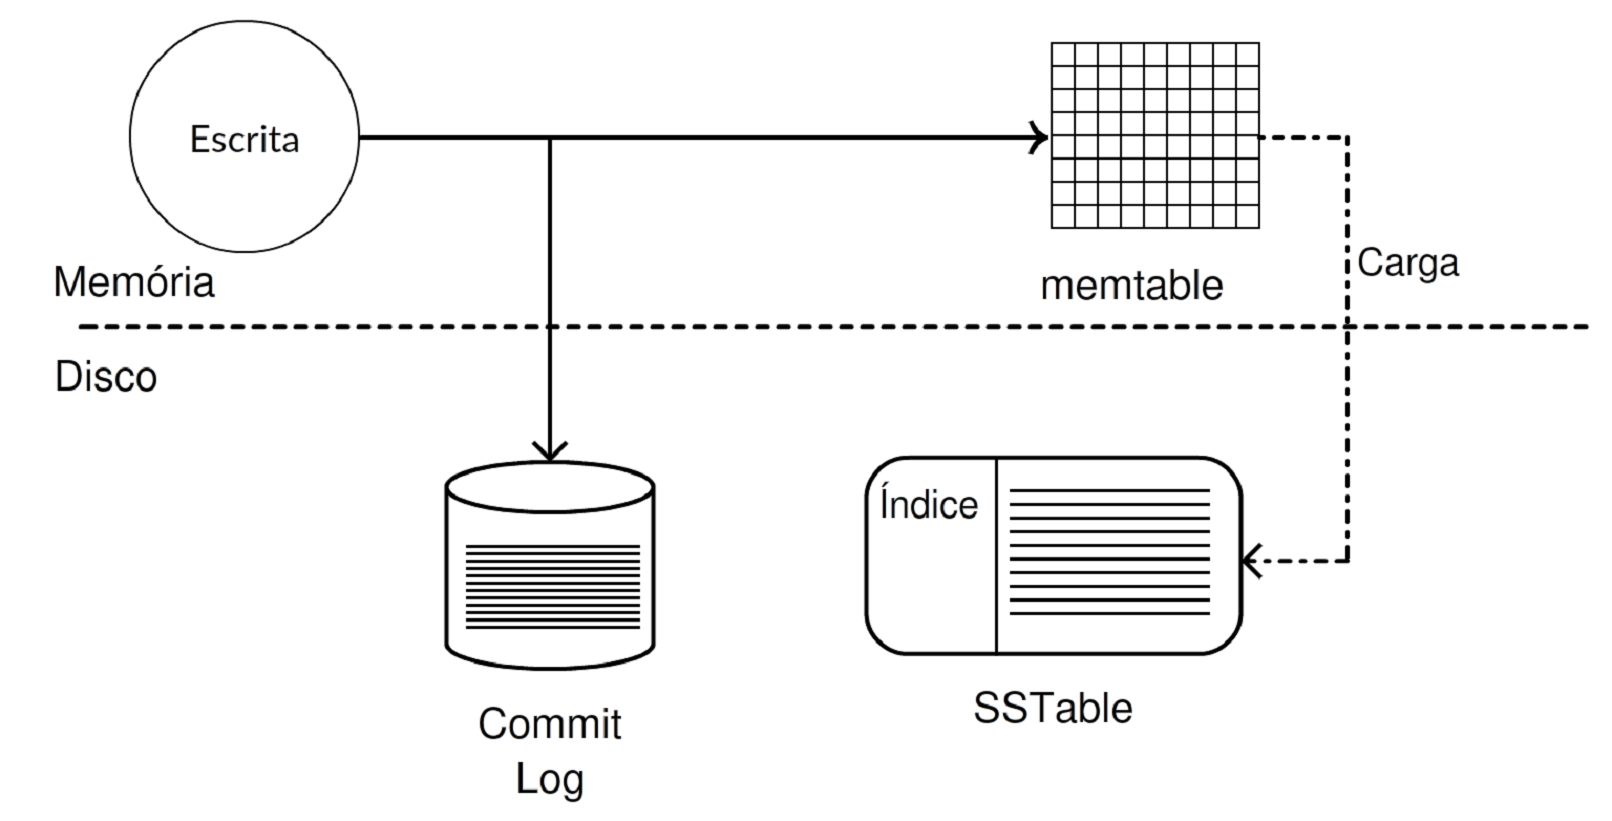
\includegraphics[width=1\textwidth]{figuras/cassandrawriteop.png}
\caption{Escrita de dados em um banco Cassandra. Adaptado de ~\cite{cassandradocs}}
\label{fig:cassandrawriteop}
\end{figure}

Ao se realizar uma operação de leitura o Cassandra inicialmente busca a informação solicitada na \emph{memtable}. Caso não seja encontrada, é realizada uma busca na \emph{cache} de linha, uma estrutura em memória que armazena em memória um subconjunto da partição de dados armazenado nas \emph{SSTable}. Se a \emph{cache} de linha não possuir o dado em específico, é realizada uma consulta no \emph{Bloom Filter} associado à \emph{SSTable} em questão~\cite{cassandradocs}. 

Um \emph{Bloom Filter} é um algoritmo de busca não determinístico que testa de forma rápida se um elemento faz parte de um conjunto. É dito não determinístico pois é possível obter falso positivos em uma consulta, mas não falso negativos. Em outras palavras, um \emph{Bloom Filter} garante que um dado não está presente no conjunto, mas se ele indicar que o dado está presente uma consulta deve ser realizada no conjunto para se obter uma confirmação~\cite{cassandraguide}.

Caso o \emph{Bloom Filter} indique que o dado pode estar presente em uma \emph{SSTable} são realizadas algumas operações de busca de índice para encontrar sua localização, e o dado é então retornado na consulta~\cite{cassandradocs}.

\subsection{Distribuição de Dados}
Distribuição e replicação de dados no Cassandra são conceitos que se conectam. Devido ao fato de um \emph{cluster} Cassandra ser uma rede sem hierarquia entre nós, o sistema faz cópias (ou réplicas) dos dados e as distribui entre os nós. Esses dados são organizados por tabelas identificadas por chaves primárias, que determinam em que nó desse \emph{cluster} esse dado será armazenado~\cite{cassandradocs}.

O Cassandra utiliza um sistema de \emph{hashing} consistente, que permite a distribuição de dados no \emph{cluster} de forma a minimizar a reorganização do mesmo quando nós são inseridos ou removidos. O \emph{hashing} consistente particiona os dados baseados em uma chave de partição (\emph{partition key}), que é obtida do primeiro componente da chave primária de cada tabela. Dessa forma, cada nó em um \emph{cluster} é responsável por um intervalo de dados baseado nesse mapeamento~\cite{cassandradocs}.

A partir de sua versão 1.2 o Cassandra permite que a cada nó físico seja atribuído mais de um \emph{token}, que determina a posição desse nó no anel e a porção de dados de que ele é responsável. Esse novo paradigma de distribuição foi chamado de nós virtuais (\emph{virtual nodes} ou \emph{vnodes}).
Nós virtuais permitem que cada nó possua um grande número de pequenos intervalos de partições distribuídos pelo \emph{cluster}~\cite{cassandradocs}.

A figura \ref{fig:vnodes} mostra a distribuição de nós em um anel, comparando uma arquitetura sem nós virtuais com uma utilizando nós virtuais. 

Na primeira parte da figura a cada nó é atribuído um único \emph{token} que representa sua posição no anel. Cada nó armazena dados determinados pelo mapeamento da chave de partição para um valor no intervalo entre o nó anterior e o valor do \emph{token}. Cada nó também possui réplicas de cada linha de outros nós do \emph{cluster}. 

Na segunda parte da figura, nós virtuais são selecionados aleatoriamente e de forma não contígua. A posição de uma linha é determinada pelo mapeamento da chave de partição dentro de vários pequenos intervalos de partição pertencentes a cada nó~\cite{cassandradocs}.


\subsection*{Replicação de Dados}
O Cassandra armazena réplicas de dados em múltiplos nós para garantir confiabilidade e tolerância a falhas. A estratégia de replicação determina em que nós as cópias serão armazenadas. O número de cópias em um \emph{cluster} é chamado fator de replicação. Se um fator de replicação um é utilizado, existe apenas uma copia de cada linha no \emph{cluster}, ou seja, se o nó contendo essa linha cai, a linha não pode ser acessada. Todas as rélicas são igualmente importantes, não existe uma réplica mestre ou primária. Como regra geral, o fator de replicação não deve exceder o número de nós no \emph{cluster}. É possível, porém, aumentar o fator de replicação e inserir o número desejado de nós posteriormente~\cite{cassandradocs}.

Existem duas estratégias de replicação:
\begin{itemize}
\item \textbf{\emph{SimpleStrategy}} é utilizada para um único \emph{data center} e um único \emph{rack}. A primeira réplica de um nó é determinada pelo particionador, e réplicas adicionais são posicionadas nos próximos nós no anel em sentido horário, sem se considerar a topologia do sistema. 
\item \textbf{\emph{NetworkTopologyStrategy}} deve ser utilizada quando se tem, ou se planeja ter, um \emph{cluster} distribuído em vários \emph{data centers}. Essa estratégia especifica quantas réplicas se deseja em cada \emph{data center}. As réplicas são inseridas em um mesmo \emph{data center} caminhando-se no anel em sentido horário até se alcançar o primeiro nó em outro \emph{rack}. A \emph{NetworkTopologyStrategy} tenta colocar réplicas em \emph{racks} distintos, por entender que nós em um mesmo \emph{rack} frequentemente falham ao mesmo tempo por problemas de energia, resfriamento ou falhas na rede.
\end{itemize}

Estratégias de replicação são definidas por \emph{keyspace} e definidas durante sua criação~\cite{cassandradocs}.

~\begin{figure}[!htb]
\centering
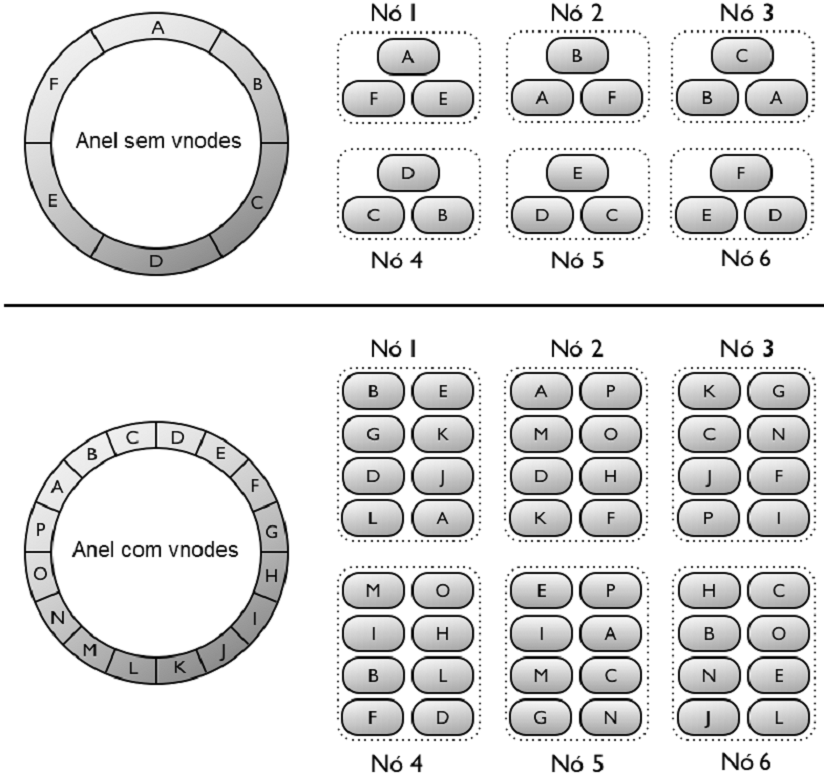
\includegraphics[width=1\textwidth]{figuras/vnodes.png}
\caption{Distribuição de nós em um anel. Adaptado de ~\cite{cassandradocs}}
\label{fig:vnodes}
\end{figure}

\subsection*{Particionadores}
Um particionador determina de que forma os dados e suas réplicas serão distribuídos no \emph{cluster}. Basicamente um particionador é uma função que deriva um \emph{token} a partir de uma chave de partição, geralmente por meio de um mapeamento (\emph{hash}). Cada linha de dados é então distribuída no \emph{cluster} de acordo com o valor desse token. 

O Cassandra fornece três particionadores, que podem ser definidos no arquivo de configuração principal do Cassandra, o \emph{cassandra.yaml}. São ele:

\begin{itemize}
\item \textbf{\emph{Murmur3Partitioner}} distribui os dados de forma uniforme no \emph{cluster}, de acordo com valores da função \emph{hash} \emph{MurmurHash}, que cria valores de 64 bits com a chave de partição. É o particionador padrão e fornece um desempenho melhor que o do \emph{RandomPartitioner};


\item \textbf{\emph{RandomPartitioner}} também distribui os dados uniformemente no \emph{cluster}, porém com a utilização de uma função \emph{hash} MD5. Essa é uma função criptográfica com um tempo de execução mais longo que a \emph{MurmurHash}. Como o Cassandra não exige um \emph{hash} criptográfico, o particionador \emph{RandomPartioner} reduz o desempenho do Cassandra de 3 a 5 vezes em comparação ao \emph{MurmurPartitioner}

\item \textbf{\emph{ByteOrderedPartitioner}} distribui os nós no \emph{cluster} em ordem alfabética. É utilizado quando se deseja um particionamento ordenado, porém causa problemas de dificuldade de balanceamento de carga, pontos quentes em escritas sequenciais e balanceamento desigual de carga para múltiplas tabelas. É incluído no Cassandra por razões de retrocompatibilidade.
\end{itemize}

Tanto o \emph{MurmurPartitioner} quanto o \emph{RandomPartitioner} utilizam to\emph{tokens} para auxiliar na designação de porções iguais de dados para cada nó e na distribuição de forma uniforme desses dados a partir de todos as tabelas do anel ou de outros agrupamentos, como um \emph{keyspace}.
  % \chapter{Data Warehouse}

O crescimento no volume e complexidade dos dados e informações nas últimas décadas tem levado organizações, empresas e governos a buscarem ferramentas que auxiliem na tomada de decisões de forma rapida e estatégica. Informação é um dos recursos mais importantes em qualquer organização, e em geral é utilizada para dois propósitos: registro operacional e tomada de decisões~\cite{dwkimball}. 

A abordagem que vem se destacando como uma das mais promissoras no auxílio à tomada de decisões é o modelo conhecido como \emph{Data Warehouse}.

\section{Definição}

  % ...

  \postextual
  \bibliographystyle{plain}
  \bibliography{bibliografia}

\end{document}
